\begin{figure}[H]
  \begin{center}
    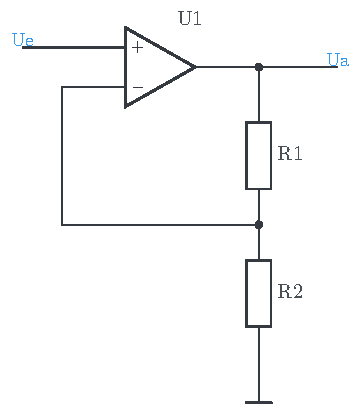
\includegraphics[height=0.618\textwidth]{circuits/nichtinv_verst.pdf}
    \end{center}
    \caption{Nichtinvertierende Verstärkerschaltung}
 \end{figure}

 \begin{gather*}
  U_a = V_0(U_p-U_n)\\
  U_a = V_0(U_e-U_n)\\
  U_n = U_a \frac{R_1}{R_1+R_2}\\
  U_a = V_0 (U_e - U_a \frac{R_1}{R_1 + R_2})\\
  U_a (1 + V_0 \frac{R_1}{R_1 + R_2}) = V_0 U_e\\
  \frac{U_a}{U_e} = V = \frac{V_0}{1 + V_0 \frac{R_1}{R_1+R_2}}\\
  \intertext{für $V_0 \rightarrow \infty$}
  V = \frac{R_1 + R_2}{R_1} = 1 + \frac{R_2}{R_1}
\end{gather*}

